\documentclass{beamer}
\usepackage[latin1]{inputenc}
\usefonttheme{serif} 
\usefonttheme{structuresmallcapsserif} 

\usetheme{Luebeck}

\usecolortheme[named=magenta]{structure}
\beamertemplatenavigationsymbolsempty
\setbeamertemplate{bibliography item}[text]
\title[Helmholtz]{Helmholtz}
\subtitle{Finite Element Method project}
\author{Hannu, Juho, Samu}


\date{April 2, 2015}



\begin{document}

\begin{frame}
\titlepage
\end{frame}

\begin{frame}{Introduction}
\begin{itemize}
\item Consider the wave equation $(\nabla^2 - \frac{1}{c^2} \frac{\partial^2}{\partial t^2})\psi(\mathbf{r}, t) = 0$. 
\item Assume that $\psi$ is separable: $\psi(\mathbf{r}, t) = u(\mathbf{r})T(t)$. 
\item Substitute to the wave equation to get $\frac{\nabla^2 u}{u} = \frac{1}{c^2 T} \frac{d^2 T}{dt^2}$. 
\item The different sides of the equation are independent. Thus, they need to be equal to the same constant, say $-k^2$.
\item Hence, we obtain for the spatial part the homogeneous Helmholtz equation, $\Delta u + k^2 u = 0$.
\item We will use a Robin boundary condition, noting that $u$ is complex-valued.
\end{itemize}
\end{frame}


\begin{frame}{Problem}

\begin{definition}[Helmholtz equation]
\[ \begin{cases}
\Delta u + k^2 u = f \ \mathrm{in} \ \Omega \\ \frac{\partial u}{\partial n} + iku = g \ \mathrm{on} \ \partial \Omega.
\end{cases} \]
\end{definition}
\begin{itemize}
\item The Sommerfeld radiation condition is useful: it describes the boundary conditions while no external sources are present.
\item In 2D, as $r \rightarrow \infty$, $u = O(\frac{1}{\sqrt{r}})$ and $g = O(\frac{1}{\sqrt{r}})$. % insert source
\item Using Green's first identity, we get the weak form of the problem.
\end{itemize}
\begin{definition}[Weak form]
$(\nabla u, \nabla v)_{\Omega} - k^2(u, v)_{\Omega} + ik(u, v)_{\partial \Omega} = -(f, v)_{\Omega} + (g, v)_{\partial \Omega}.$
\end{definition}
\end{frame}
% http://www.encyclopediaofmath.org/index.php/Radiation_conditions

\begin{frame}{Solver implementation}
 
\begin{itemize}
 \item A circular domain is used, so that the normal of the boundary is always in the radial direction.
 \item The $\Omega$ parts can be solved in 2D using the $simple\_assembly$ that was in use during the course.
 \item The $\partial \Omega$ parts require the usage of a boundary 1D FEM integral.
 \item These resemble the 1D integral that was encountered in one homework problem.
 \item $ik(u, v)_{\partial \Omega}$ leads to a boundary system matrix similar to that of $(\nabla u, \nabla v)_{\Omega} - k^2(u, v)_{\Omega}$.
 \item $(g, v)_{\partial \Omega}$ leads to a boundary load vector similar to that of $-(f, v)_{\Omega}$.
\end{itemize}

\end{frame}

\begin{frame}{Solver testing}
\begin{itemize}
 \item A toy problem: simulate a scaled delta-function with $H(1-r^2)$ (Heaviside).
 \item Assumed that the Sommerfeld radiation condition is approximately valid already with a quite small $r$.
\end{itemize}
 \begin{center}
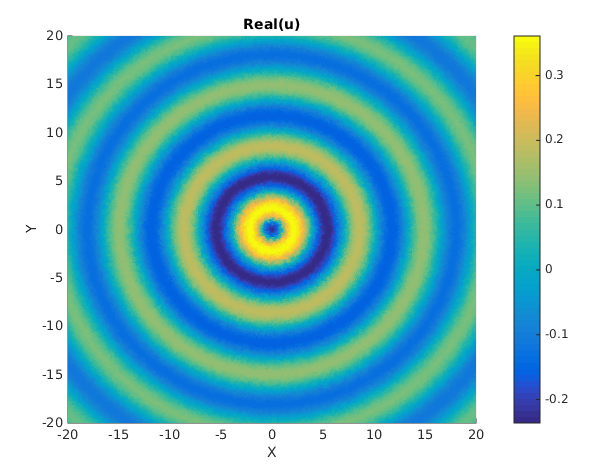
\includegraphics[width=.5\textwidth]{delta_real.png}%
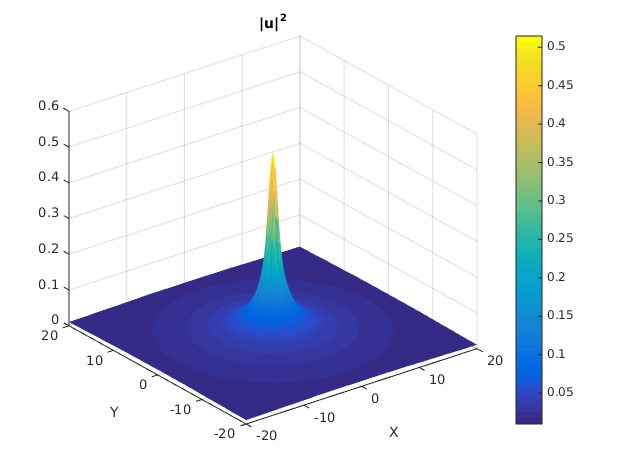
\includegraphics[width=.5\textwidth]{delta_abs2.png}
\end{center}
\end{frame}

\begin{frame}{Plane waves and errors}
\begin{columns}
  \begin{column}{0.39\textwidth}
    \begin{itemize}
    \item Since the solver seems to be working, we should do error studies.
    \item It is hard to come up with a good, general load $f$.
    \item A good alternative: use an external source - a plane wave propagating in the $x$-direction.
    \end{itemize}        
  \end{column}
  \begin{column}{0.61\textwidth}
    \begin{center}
    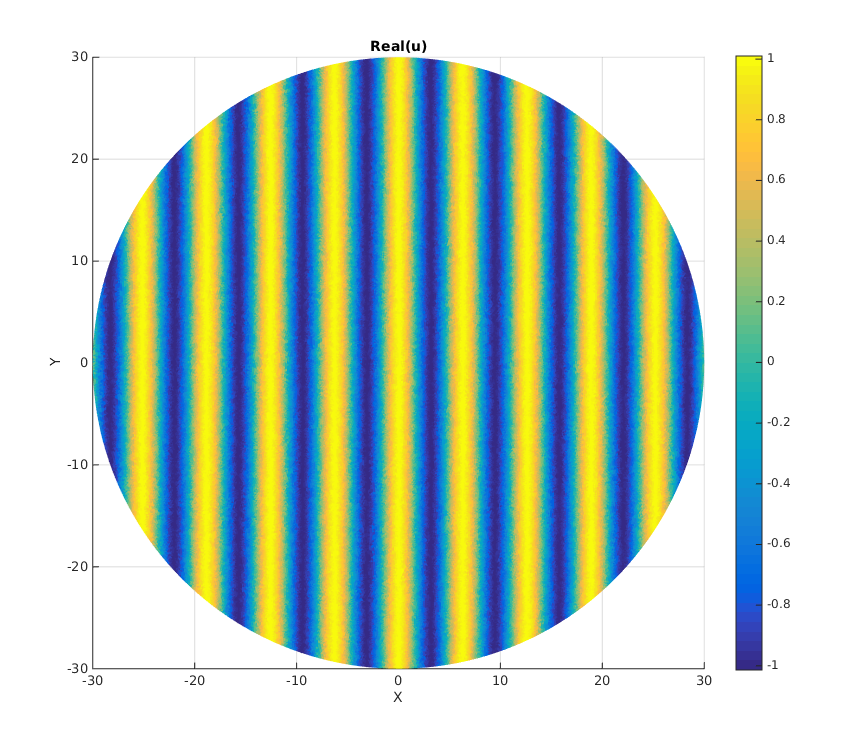
\includegraphics[width=\textwidth]{planewave_real.png}
    \begin{itemize}
    \item A generic plane wave has the form $u = e^{-ikx}$.
    \end{itemize}
    \end{center}
  \end{column}
\end{columns}
\end{frame}

\begin{frame}{Basics of error analysis}
 \begin{itemize}
  \item The external plane wave source is added to $g$ using the explicit form of the boundary condition.
  \item Basically there are three parameters that can affect the errors
  \begin{itemize}
  \item The radius of the domain, $r$: this is only important in the sense that the Sommerfeld radiation condition
  should be correct for the used $k$ (large enough $r$).
  \item The maximal edge length of the FEM mesh, $h$: this should be small enough as compared to the wavelength,
  $2\pi/k$.
  \item The constant $k$ i.e. the wave number: the relationships to other parameters mentioned above.
  \end{itemize}
  \item It is possible to keep $r$ constant and use it for setting the length scale/units of the system.
 \end{itemize}
\end{frame}

\begin{frame}{H1 errors}
 \begin{itemize}
  \item When the H1 error is plotted as a function of $h$, there is a 'knee' in the error plot for each $k$.
  \item This is found approximately at a constant value of $kh$, which is with the used parameter values located at $kh \in [2,3]$.
 \end{itemize}

\end{frame}

\begin{frame}{Conclusions}
 Diibadaaba
\end{frame}


\end{document}